\chapter{Vergleich der Einkommensverteilungen anhand mehrerer Indikatoren}

Im Folgenden soll die Einkommensverteilung in Deutschland mit der weltweiten Einkommensverteilung anhand mehrerer Indikatoren verglichen werden. Die Indizes, die hierfür verwendet werden, sind das Verhältnis des Durchschnittseinkommens der reichsten 10\% zum Durchschnittseinkommens der ärmsten 50\%, der Gini-Koeffizient und der Bevölkerungsanteil mit einem Einkommen unterhalb der Armutsgrenze. Durch die Auswertung dieser Kennzahlen soll ein umfassendes Verständnis über die Einkommensverteilung Deutschlands im weltweiten Vergleich geschaffen werden.
\section{T10/ B50 Einkommensverhältnis}

Zuerst wird das gewichtete Verhältnis des Durchschnittseinkommens der reichsten 10\% zum Durchschnittseinkommen der ärmsten 50\% in Deutschland und auf globaler Ebene von 1900 bis 2020 betrachtet (Im Folgenden als ''T10/B50'' abgekürzt). Es gibt an, wie viel die reichsten 10\% im Vergleich zu den ärmsten 50\% verdienen gewichtet nach der absoluten Größe der Gruppen. Je höher der Wert, desto ungleicher sind die Einkommen verteilt. \footcite[Vgl.][S. 31]{wir_2022}

\begin{figure}[H]
    \centering
    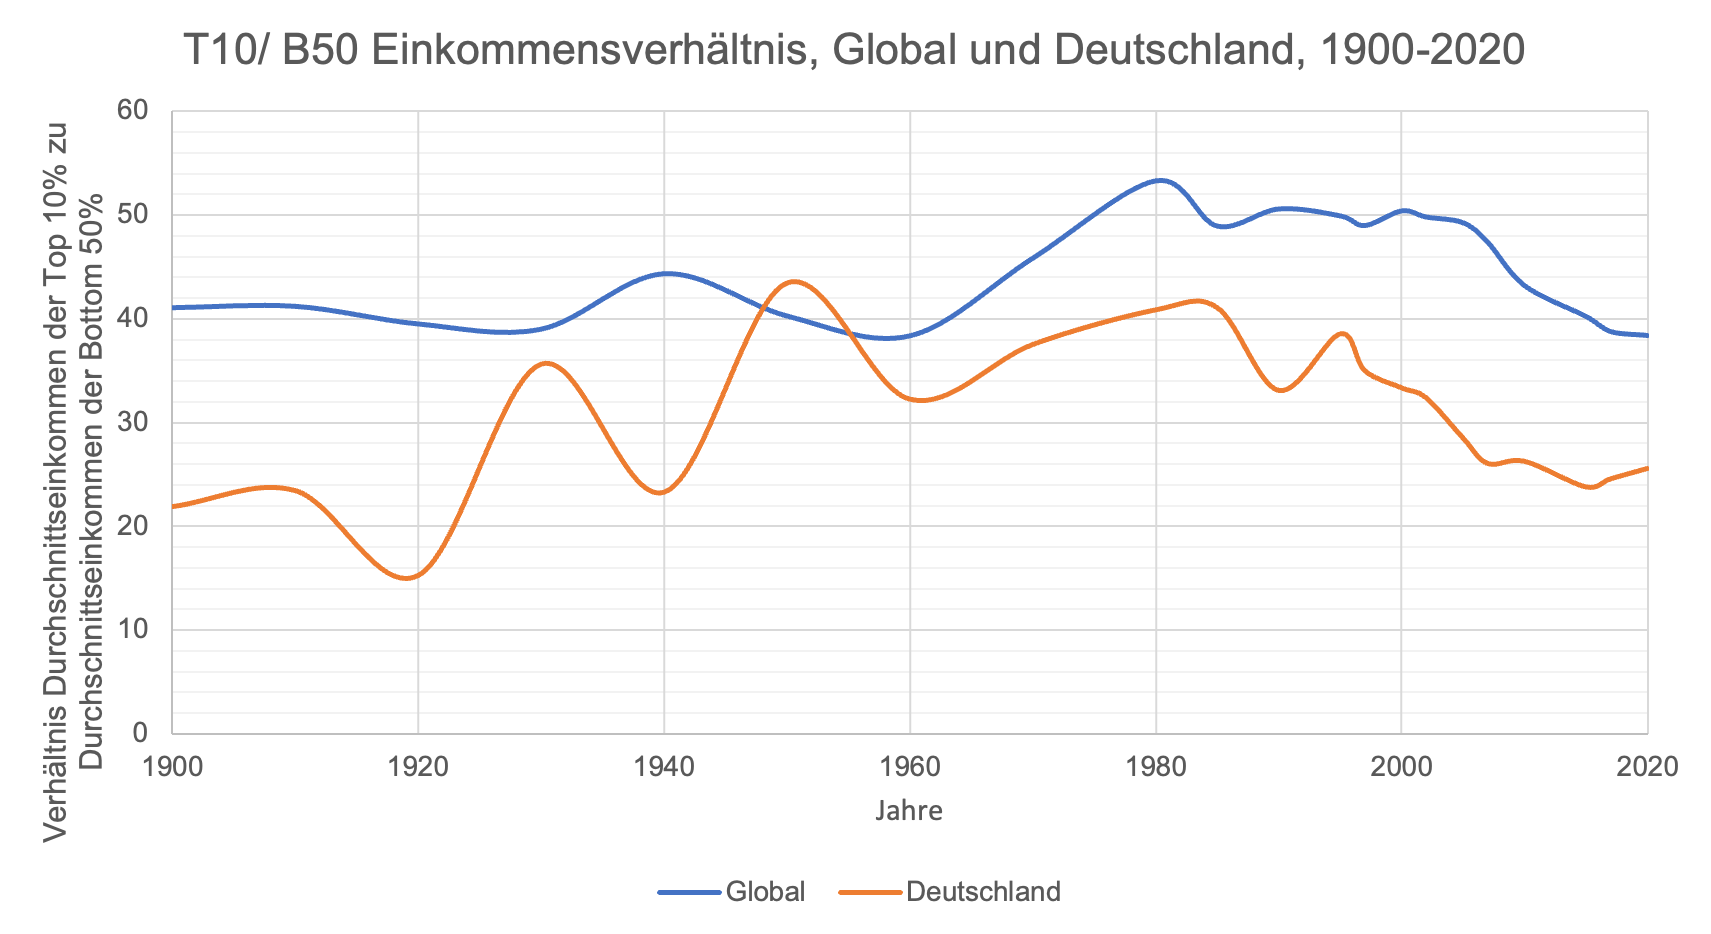
\includegraphics[height=8.15cm]{Bilder/T10B50-Ratio.png}
    \caption[T10/B50-Verhältnis, Deutschland und global, 1900-2020]{gewichtetes Verhältnis des Durchschnittseinkommens der reichsten 10\% zum Durchschnittseinkommen der ärmsten 50\% in Deutschland und auf globaler Ebene von 1900 bis 2020. Eigene Darstellung und Berechnung. Daten abgerufen von \cite[][, S.55, 195]{wir_2022} am 01.03.2024.}
    \label{fig:iso_norm}
\end{figure}

\section{Gini-Koeffizient}

Der zweite herangezogene Indikator ist der Gini-Koeffizient. Er ist ein Maß für die (Un-)Gleichverteilung von Einkommen und Vermögen. Er kann Werte zwischen 0 und 1 annehmen, wobei 0 für eine vollkommene Gleichverteilung und 1 für eine vollkommene Ungleichverteilung steht. \footcite[Vgl.][]{gini_definition_diw_2024}

\begin{figure}[H]
    \centering
    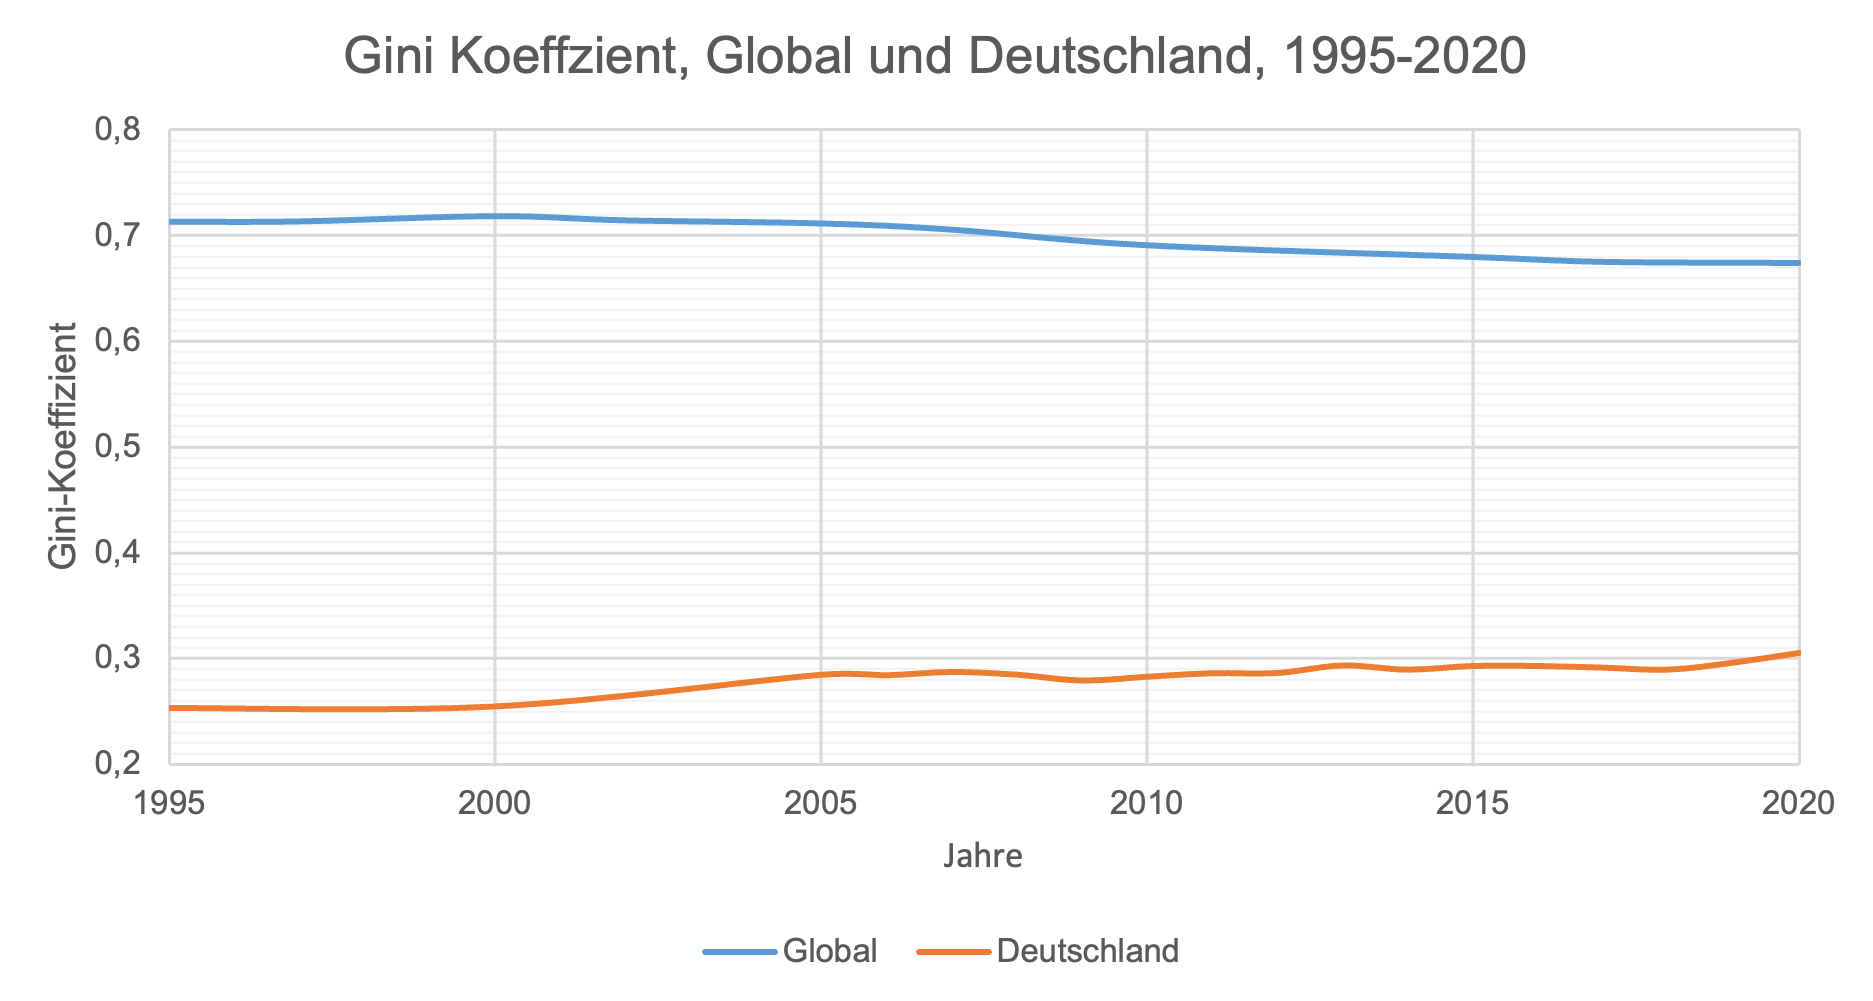
\includegraphics[height=8cm]{Bilder/Gini-Koeffizient2.png}
    \caption[Gini-Koeffizient, Deutschland und global, 1995-2020]{Gini-Koeffizient für Deutschland und auf globaler Ebene von 1995 bis 2020. Eigene Darstellung. Daten abgerufen von \cite[][, S.56 (global)]{wir_2022} und \cite[][(Deutschland)]{bmas_arb_gini_2020} am 01.03.2024.}
    \label{fig:iso_norm}
\end{figure}

\section{Bevölkerungsanteil unterhalb der Armutsgrenze}

Als letzte Kennzahl wird der Anteil der Bevölkerung mit einem Einkommen unterhalb der Armutsgrenze betrachtet. In Deutschland ist die Armutsrisikoquote bei 60\% des Medianeinkommens angesetzt. \footcite[Vgl.][]{bmas_arb_armutsrisikoquote_2023} Für die globale Betrachtung werden die jeweiligen Einkommensgrenzen, die jedes Land für sich definiert hat, verwendet. \footcite[Vgl.][]{wb_armutsquote_global_2022}

\begin{figure}[H]
    \centering
    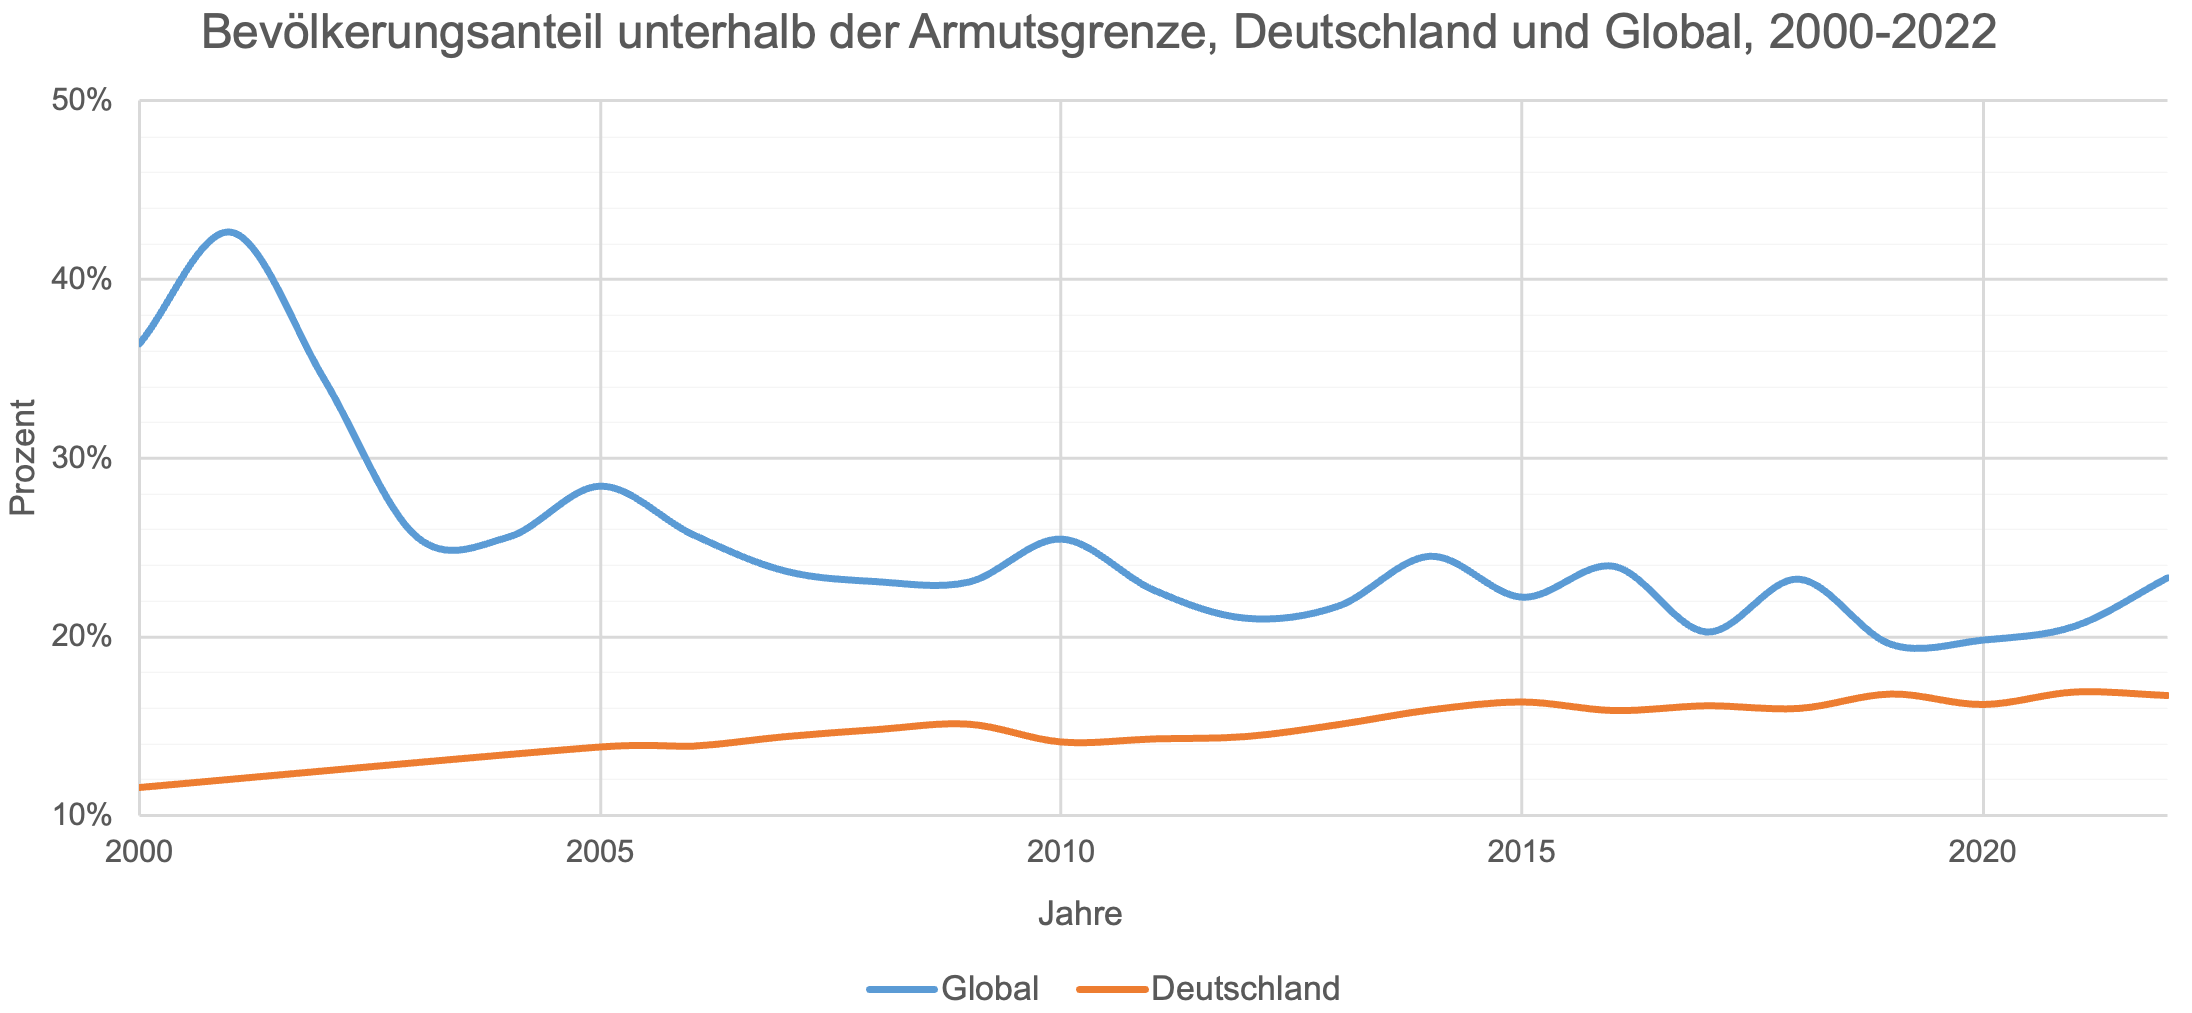
\includegraphics[height=6.9cm]{Bilder/Armutsgrenze2.png}
    \caption[Bevölkerungsanteil unterhalb der Armutsgrenze, Deutschland und global, 2000-2020]{Bevölkerungsanteil mit einem Einkommen unterhalb der Armutsgrenze in Deutschland und auf globaler Ebene von 2000 bis 2020. Eigene Darstellung und Berechnung. Daten abgerufen von \cite[][(global)]{wb_armutsquote_global_2022} und \cite[][(Deutschland)]{bmas_arb_armutsrisikoquote_2023} am 01.03.2024.}
    \label{fig:iso_norm}
\end{figure}

